\documentclass{article}
\usepackage{tikz, comment}
\usepackage{pifont}
\usepackage{fontspec}
\usetikzlibrary{arrows, decorations.markings, decorations.pathreplacing}
\begin{comment}
:Title: Not defined yet
:Tags: area using parametric equations,parametric integral formula;cycloid;arc length of a curve;area under a curve;cardioid
:Prob: 0.4738;0.4699;0.3807;0.3289;0.3261
:Author: Prof.Hu Ji-shan, HKUST
:Slug: No name yet

Description Here.........
\end{comment}
\begin{document}\centering

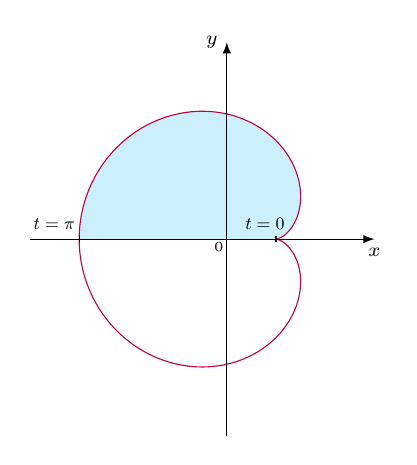
\begin{tikzpicture}[>=latex,xscale=.5*1.25, yscale=.5*1.25][font=\sf\small]

%\draw[xstep=1cm,ystep=1cm,color=gray!80] (0, -1) grid (8, 8);

\draw[purple, fill=cyan!20, samples=200, smooth, domain=0:pi, variable=\t]
plot ({2*cos(\t r) - cos(2*\t r)}, {2*sin(\t r) - sin(2*\t r)});
\draw[purple, fill=white, samples=200, smooth, domain=pi:2*pi, variable=\t]
plot ({2*cos(\t r) - cos(2*\t r)}, {2*sin(\t r) - sin(2*\t r)});

\foreach \x in {}
\draw (\x,2pt/6) -- (\x,-2pt/6)
node[anchor=north] {\tiny$\x$}
;
\draw (1,2pt/1.25) -- (1,-2pt/1.25)node[above, xshift=-4, yshift=2, scale=0.7] {$t=0$};
\draw (-3,2pt/1.25) -- (-3,-2pt/1.25)node[above, xshift=-9, yshift=2, scale=0.7] {$t=\pi$};

\foreach \x in {}
\draw (\x,2pt/2.5) -- (\x,-2pt/2.5)
node[anchor=south] {\tiny$\x$}
;
\foreach \y in {}
\draw (-2pt/6,\y) -- (2pt/6,\y)
node[anchor=east] {\tiny $\y$}
;

\draw[->] (-4, 0) -- (3, 0)node[below] {\scriptsize$x$} ;
\draw[-> ] (0, -4) -- (0, 4)node[left] {\scriptsize$y$} ;

\node[yshift=0] at (-0.2/1.25, -0.2/1.25) {\tiny$0$};

\end{tikzpicture}
\end{document}